\subsection{Configurable Evaluation Dataset Generation}
\label{sec:method_evaldataset}

\subsubsection{Three Query Types}

\textcolor{blue}{EABench does not treat evaluation cases as fixed annotations authored by hand. Instead, it derives them automatically from the generated tenant history, producing three query types that cover retrieval, reasoning, and synthesis. Needle-in-a-haystack cases ask the agent to locate a specific artifact or a very small set of artifacts without ever naming internal identifiers explicitly. Multi-step reasoning cases require the agent to follow a dependency chain across multiple modalities, such as resolving a person in one artifact and then using that reference to locate the decisive meeting or file. Deep-dive report cases ask for a coherent summary of an incident or initiative spread across several days of activity. This tripartite design ensures that evaluation does not collapse to a single notion of success.}

\begin{figure}[t]
\centering
%\resizebox{0.95\linewidth}{!}{\begin{tikzpicture}[
  font=\small,
  box/.style={draw, rounded corners=2pt, align=center, minimum height=8mm, inner sep=4pt},
  arr/.style={-{Latex[length=2mm]}, thick}
]
  \node[box, fill=cyan!8, minimum width=0.82\linewidth] (log) {
    \textbf{Tenant History and Generation Log}\\
    emails, chats, meetings, files, storyline events, user roster
  };

  \node[box, fill=green!8, minimum width=0.24\linewidth, below left=10mm and 1mm of log] (search) {
    \textbf{Needle-in-a-Haystack}\\
    artifact batches
  };
  \node[box, fill=orange!10, minimum width=0.24\linewidth, below=10mm of log] (multihop) {
    \textbf{Multi-Step Reasoning}\\
    daily event clusters
  };
  \node[box, fill=purple!10, minimum width=0.24\linewidth, below right=10mm and 1mm of log] (report) {
    \textbf{Deep-Dive Reports}\\
    3--7 day windows
  };

  \node[box, fill=yellow!10, minimum width=0.82\linewidth, below=12mm of multihop] (gt) {
    \textbf{Ground Truth Packaging}\\
    query + user\_id + weighted assertions + entity\_list
  };

  \node[box, fill=blue!8, minimum width=0.82\linewidth, below=10mm of gt] (dataset) {
    \textbf{Evaluation Dataset}\\
    unified YAML cases for runtime execution and judge scoring
  };

  \draw[arr] (log) -- (search);
  \draw[arr] (log) -- (multihop);
  \draw[arr] (log) -- (report);
  \draw[arr] (search) -- (gt);
  \draw[arr] (multihop) -- (gt);
  \draw[arr] (report) -- (gt);
  \draw[arr] (gt) -- (dataset);
\end{tikzpicture}}
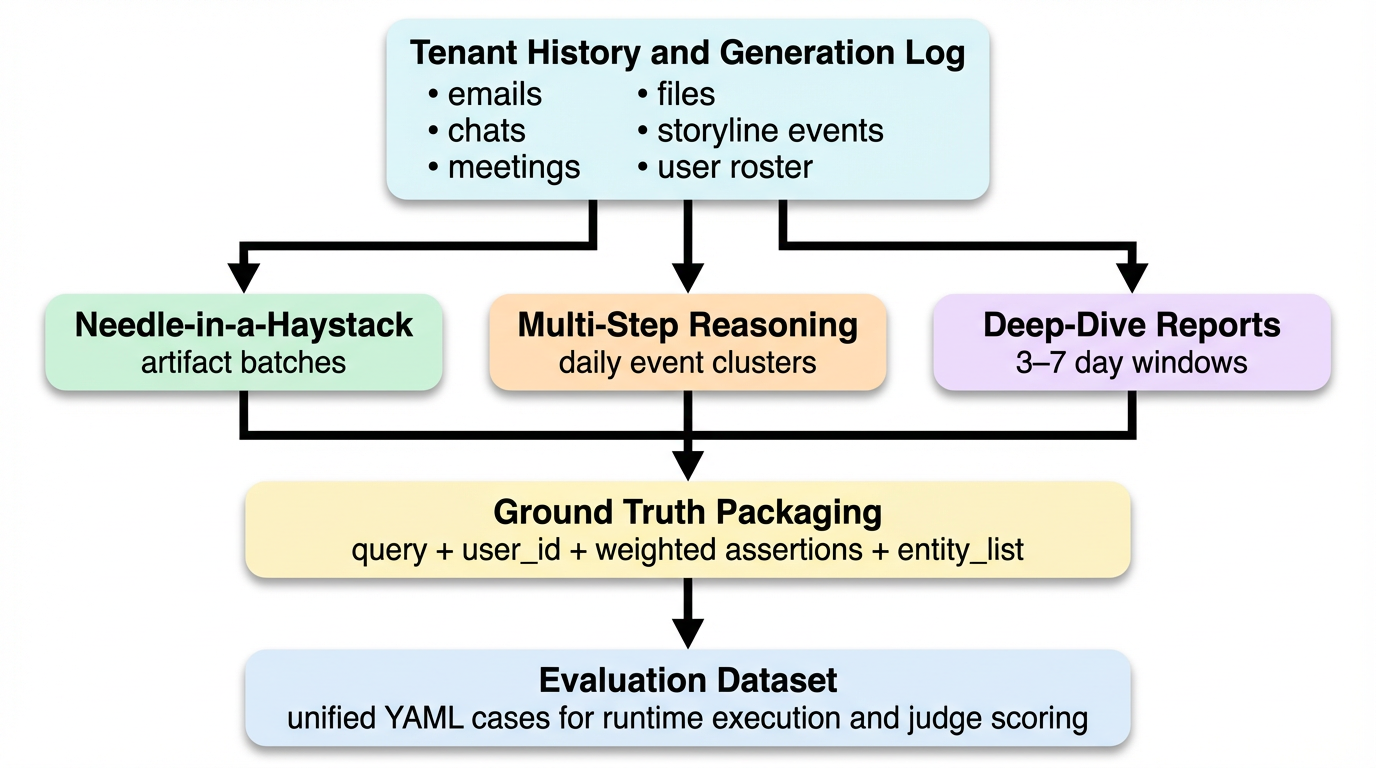
\includegraphics[width=0.7\textwidth]{figures/eval_data_generation_pipeline.png}
\caption{\textcolor{blue}{Evaluation-case generation pipeline. The same tenant history is re-sliced into retrieval, reasoning, and report-generation cases, each with explicit user context and ground truth.}}
\label{fig:eval_pipeline}
\end{figure}

\begin{table}[h]
\centering
\caption{\textcolor{blue}{Automatically generated query types in EABench.}}
\label{tab:query_types}
\small
{\color{blue}
\begin{tabular}{p{0.21\linewidth}p{0.34\linewidth}p{0.35\linewidth}}
\toprule
\textbf{Query type} & \textbf{Typical form} & \textbf{Primary benchmarked capability} \\
\midrule
Needle-in-a-haystack retrieval & Request to find a specific email, file, meeting, or message using natural constraints such as date, author, topic, or artifact type & Precision retrieval under realistic phrasing and user-level access control \\
Multi-step reasoning & Request whose answer depends on chaining evidence across multiple artifacts, often across different modalities & Decomposition, dependency tracking, and selective tool use \\
Deep-dive report generation & Request for a briefing, incident summary, or thematic report over a multi-day window & Long-form synthesis, temporal organization, and citation-grounded summarization \\
\bottomrule
\end{tabular}
}
\end{table}

\subsubsection{Ground Truth Association}

\textcolor{blue}{Every generated case carries two forms of ground truth. The first is a structured \texttt{entity\_list}, which records the concrete artifacts that a correct solution should retrieve. The second is a set of natural-language assertions that describe what the answer must contain. Each case is also bound to a specific \texttt{user\_id}, which means the case is evaluated under an explicit access-control context rather than against a globally visible corpus. This design is important because it distinguishes ``the answer is wrong'' from ``the answer is unavailable to this user.''}

\subsubsection{Assertion Generation for Fact Checking}

\textcolor{blue}{Assertions are generated automatically from the same context used to formulate the query. They are written in natural language, may be weighted by importance, and focus on factual obligations rather than stylistic preferences. A search case might require the answer to name the correct sender and subject line, while a report case might require the answer to mention the triggering event, the main decision, and the relevant date range. This representation makes evaluation robust to paraphrase while still preserving strong factual expectations.}

\subsubsection{Realism Constraints}

\textcolor{blue}{The prompts that generate cases enforce several realism constraints. Queries never mention internal artifact identifiers directly. User identities are assigned plausibly, such as recipients for emails or attendees for meetings. Multi-hop cases are only produced when the source context contains a realizable dependency chain, and report cases are grounded in contiguous event windows so that the requested narrative exists in the tenant history. These constraints matter because they prevent the generator from creating benchmark cases that are formally valid but operationally unnatural.}

\subsubsection{Generation Pipeline}

\textcolor{blue}{Case generation itself proceeds in three passes over the tenant history. The first pass shuffles artifact summaries and generates needle-in-a-haystack queries. The second pass groups events by day and proposes multi-step cases only when there are enough linked artifacts to support a dependency chain. The third pass samples 3--7 day windows and generates report requests over the resulting event clusters. By writing all cases to a single evaluation dataset with shared structure, EABench ensures that retrieval, reasoning, and report synthesis can be evaluated side by side under the same runtime and judge configuration.}